\documentclass{ximera}

\input{../../../preamble.tex}


\definecolor{fvdnavy}{HTML}{071D43}
\definecolor{fvdcyan}{HTML}{20BFC6}
\definecolor{fvdcyanlight}{HTML}{EFFCFB}
\definecolor{fvdmagenta}{HTML}{F10D69}
\definecolor{fvdmagentalight}{HTML}{FFF1F7}
\definecolor{fvdtext}{HTML}{163044}





%=================================================
% Pedagogische omgevingen
% PDF: tcolorbox
% HTML: learning-box
%=================================================

\newenvironment{voorkennis}
{%
    \ifdefined\HCode
        \HCode{%
<section class="learning-box learning-box--prior">
<div class="learning-box__header">
<span class="learning-box__icon" aria-hidden="true"></span>
<span class="learning-box__title">Voorkennis</span>
</div>
<div class="learning-box__content">
        }%
        \begin{itemize}
    \else
       \begin{tcolorbox}[
    enhanced,
    breakable,
    colback=fvdcyanlight,
    colframe=fvdcyan,
    coltext=fvdtext,
    boxrule=0.5pt,
    leftrule=4pt,
    arc=4mm,
    outer arc=4mm,
    left=7mm,
    right=6mm,
    top=5mm,
    bottom=5mm,
    before skip=6mm,
    after skip=6mm,
    title=Voorkennis,
    coltitle=fvdcyan,
    fonttitle=\bfseries\Large,
    attach title to upper={\par\smallskip},
    boxed title style={
        empty,
        left=0mm,
        right=0mm,
        top=0mm,
        bottom=0mm
    },
    overlay={
        \draw[
            fvdcyan,
            line width=0.5pt
        ]
        ([xshift=42mm,yshift=-13mm]frame.north west)
        --
        ([xshift=-7mm,yshift=-13mm]frame.north east);
    }
]
        \begin{itemize}
    \fi
}
{%
    \end{itemize}
    \ifdefined\HCode
        \HCode{%
</div>
</section>
        }%
    \else
        \end{tcolorbox}
    \fi
}


\newenvironment{leerdoelen}
{%
    \ifdefined\HCode
        \HCode{%
<section class="learning-box learning-box--goals">
<div class="learning-box__header">
<span class="learning-box__icon" aria-hidden="true"></span>
<span class="learning-box__title">Leerdoelen</span>
</div>
<div class="learning-box__content">
        }%
        \begin{itemize}
    \else
\begin{tcolorbox}[
    enhanced,
    breakable,
    colback=fvdmagentalight,
    colframe=fvdmagenta,
    coltext=fvdtext,
    boxrule=0.5pt,
    leftrule=4pt,
    arc=4mm,
    outer arc=4mm,
    left=7mm,
    right=6mm,
    top=5mm,
    bottom=5mm,
    before skip=6mm,
    after skip=6mm,
    title=Leerdoelen,
    coltitle=fvdmagenta,
    fonttitle=\bfseries\Large,
    attach title to upper={\par\smallskip},
    boxed title style={
        empty,
        left=0mm,
        right=0mm,
        top=0mm,
        bottom=0mm
    },
    overlay={
        \draw[
            fvdmagenta,
            line width=0.5pt
        ]
        ([xshift=42mm,yshift=-13mm]frame.north west)
        --
        ([xshift=-7mm,yshift=-13mm]frame.north east);
    }
]
        \begin{itemize}
    \fi
}
{%
    \end{itemize}
    \ifdefined\HCode
        \HCode{%
</div>
</section>
        }%
    \else
        \end{tcolorbox}
    \fi
}


\addPrintStyle{../../..}

\title{Oefeningen --- Oppervlakte als som van kleine stukjes}
\author{Ingmar Herreman}

\begin{document}

% FVD_CHAPTER_DATA_START
% Automatisch gegenereerd uit index.tex.
% Niet handmatig aanpassen.
\fvdchapterdata{2}{Van oppervlakte naar integraal}{1}
% FVD_CHAPTER_DATA_END











\maketitle

\FVDbeginExercises


% ============================================================
% BASIS
% ============================================================




% ------------------------------------------------------------
% OEFENING 1
% ------------------------------------------------------------

\begin{oefening}[Opdelen in gekende figuren]{\oefB\ESS}

Bereken de gewone oppervlakte van het gekleurde gebied.

\begin{center}
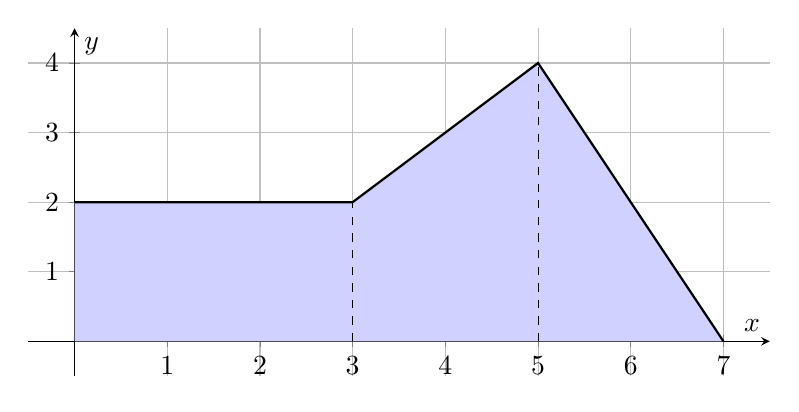
\begin{tikzpicture}
\begin{axis}[
    axis lines=middle,
    xmin=-0.5, xmax=7.5,
    ymin=-0.5, ymax=4.5,
    xlabel={$x$},
    ylabel={$y$},
    xtick={0,1,...,7},
    ytick={0,1,...,4},
    grid=both,
    width=11cm,
    height=6cm
]
    \draw[fill=blue!18,draw=none]
        (axis cs:0,0)--(axis cs:0,2)--(axis cs:3,2)--(axis cs:5,4)--(axis cs:7,0)--cycle;
    \addplot[black,thick] coordinates {(0,2) (3,2) (5,4) (7,0)};
    \draw[dashed] (axis cs:3,0)--(axis cs:3,2);
    \draw[dashed] (axis cs:5,0)--(axis cs:5,4);
\end{axis}
\end{tikzpicture}
\end{center}

\begin{oplossing}

We delen het gekleurde gebied op in drie eenvoudige delen.

Het eerste deel is een rechthoek met breedte \(3\) en hoogte \(2\):

\[
S_1=3\cdot2=6.
\]

Het tweede deel is een trapezium met evenwijdige zijden \(2\) en \(4\)
en breedte \(2\):

\[
S_2=\frac{2+4}{2}\cdot2=6.
\]

Het derde deel is een driehoek met basis \(2\) en hoogte \(4\):

\[
S_3=\frac12\cdot2\cdot4=4.
\]

Alle delen liggen boven de \(x\)-as, dus we tellen de gewone
oppervlakten op:

\[
S_{\mathrm{opp}}
=
S_1+S_2+S_3
=
6+6+4
=
\boxed{16}.
\]

\end{oplossing}

\end{oefening}


% ------------------------------------------------------------
% OEFENING 2
% ------------------------------------------------------------

\begin{oefening}[Gewone of georiënteerde oppervlakte?]{\oefB\ESS}

Een grafiek begrenst boven de \(x\)-as een gebied met oppervlakte \(8\)
en onder de \(x\)-as een gebied met oppervlakte \(3\).

\begin{question}
Bepaal de totale gewone oppervlakte.

\begin{oplossing}

Bij de gewone oppervlakte worden alle gebieden positief geteld,
ongeacht of ze boven of onder de \(x\)-as liggen.

Daarom

\[
S_{\mathrm{opp}}
=
8+3
=
\boxed{11}.
\]

\end{oplossing}
\end{question}

\begin{question}
Bepaal de georiënteerde oppervlakte.

\begin{oplossing}

Het gebied boven de \(x\)-as levert een positieve bijdrage van \(8\).
Het gebied onder de \(x\)-as levert een negatieve bijdrage van \(-3\).

Dus

\[
S_{\mathrm{geo}}
=
8-3
=
\boxed{5}.
\]

\end{oplossing}
\end{question}

\begin{question}
Leg in woorden uit waarom beide antwoorden verschillend zijn.

\begin{oplossing}

Bij de gewone oppervlakte telt alleen de grootte van elk gebied. Daarom
worden alle gebieden positief opgeteld.

Bij de georiënteerde oppervlakte speelt ook de ligging ten opzichte van
de \(x\)-as een rol:

\begin{itemize}
    \item boven de \(x\)-as: positieve bijdrage;
    \item onder de \(x\)-as: negatieve bijdrage.
\end{itemize}

Daarom krijgen we verschillende antwoorden.

\end{oplossing}
\end{question}

\end{oefening}


% ------------------------------------------------------------
% OEFENING 3
% ------------------------------------------------------------

\begin{oefening}[Georiënteerde oppervlakte uit een grafiek]{\oefB\ESS}

Bereken de georiënteerde oppervlakte van het gekleurde gebied.

\begin{center}
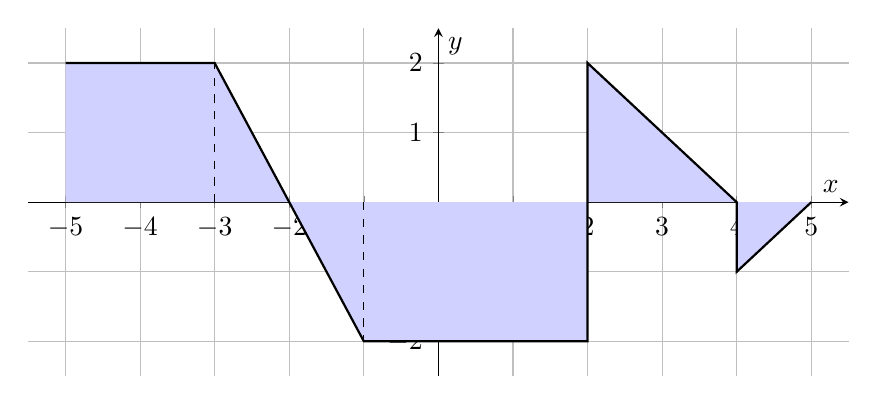
\begin{tikzpicture}
\begin{axis}[
    axis lines=middle,
    xmin=-5.5, xmax=5.5,
    ymin=-2.5, ymax=2.5,
    xlabel={$x$},
    ylabel={$y$},
    xtick={-5,-4,...,5},
    ytick={-2,-1,0,1,2},
    grid=both,
    width=12cm,
    height=6cm
]
    \draw[fill=blue!18,draw=none]
        (axis cs:-5,0)--(axis cs:-5,2)--(axis cs:-3,2)--(axis cs:-2,0)--cycle;
    \draw[fill=blue!18,draw=none]
        (axis cs:-2,0)--(axis cs:-1,-2)--(axis cs:2,-2)--(axis cs:2,0)--cycle;
    \draw[fill=blue!18,draw=none]
        (axis cs:2,0)--(axis cs:2,2)--(axis cs:4,0)--cycle;
    \draw[fill=blue!18,draw=none]
        (axis cs:4,0)--(axis cs:5,0)--(axis cs:4,-1)--cycle;

    \addplot[black,thick] coordinates {
        (-5,2) (-3,2) (-2,0) (-1,-2) (2,-2) (2,2) (4,0) (4,-1) (5,0)
    };
    \draw[dashed] (axis cs:-3,0)--(axis cs:-3,2);
    \draw[dashed] (axis cs:-1,0)--(axis cs:-1,-2);
\end{axis}
\end{tikzpicture}
\end{center}

\begin{oplossing}

We bepalen eerst de gewone oppervlakte van elk deelgebied.

Boven de \(x\)-as liggen een rechthoek met oppervlakte

\[
2\cdot2=4,
\]

een driehoek met oppervlakte

\[
\frac12\cdot1\cdot2=1,
\]

en rechts nog een driehoek met oppervlakte

\[
\frac12\cdot2\cdot2=2.
\]

Onder de \(x\)-as liggen een driehoek met oppervlakte

\[
\frac12\cdot1\cdot2=1,
\]

een rechthoek met oppervlakte

\[
3\cdot2=6,
\]

en een kleine driehoek met oppervlakte

\[
\frac12\cdot1\cdot1=\frac12.
\]

Voor de georiënteerde oppervlakte krijgen de gebieden onder de
\(x\)-as een minteken:

\[
S_{\mathrm{geo}}
=
4+1-1-6+2-\frac12
=
\boxed{-\frac12}.
\]

Het negatieve resultaat betekent dat de totale negatieve bijdrage net
iets groter is dan de totale positieve bijdrage.

\end{oplossing}

\end{oefening}


% ------------------------------------------------------------
% OEFENING 4
% ------------------------------------------------------------

\begin{oefening}[Een onbekend gebied]{\oefB\ESS}

Een grafiek begrenst drie gebieden met de \(x\)-as.

Het eerste gebied ligt boven de as en heeft oppervlakte \(7\).
Het tweede gebied ligt onder de as en heeft oppervlakte \(4\).
Het derde gebied ligt boven de as en heeft onbekende oppervlakte \(A\).

De totale georiënteerde oppervlakte is \(10\).

Bepaal \(A\).

\begin{oplossing}

De gebieden boven de \(x\)-as leveren positieve bijdragen; het gebied
onder de \(x\)-as levert een negatieve bijdrage.

Daarom

\[
7-4+A=10.
\]

Dus

\[
3+A=10
\]

en bijgevolg

\[
\boxed{A=7}.
\]

\end{oplossing}

\end{oefening}


% ------------------------------------------------------------
% OEFENING 5
% ------------------------------------------------------------

\begin{oefening}[Wanneer is de georiënteerde oppervlakte nul?]{\oefB\ESS}

Een gebied boven de \(x\)-as heeft oppervlakte \(12\).

Hoe groot moet de totale gewone oppervlakte van alle gebieden onder de
\(x\)-as zijn opdat de georiënteerde oppervlakte nul zou zijn?

\begin{oplossing}

Het gebied boven de \(x\)-as levert een positieve bijdrage van \(12\).

Noem de totale gewone oppervlakte onder de \(x\)-as \(S_-\). Die
gebieden leveren samen een negatieve bijdrage.

Voor de georiënteerde oppervlakte geldt

\[
S_{\mathrm{geo}}=12-S_-.
\]

We willen

\[
S_{\mathrm{geo}}=0.
\]

Dus

\[
12-S_-=0,
\]

zodat

\[
\boxed{S_-=12}.
\]

De totale oppervlakte onder de \(x\)-as moet dus even groot zijn als
de oppervlakte boven de \(x\)-as.

\end{oplossing}

\end{oefening}


% ============================================================
% VERDIEPING
% ============================================================



% ------------------------------------------------------------
% OEFENING 6
% ------------------------------------------------------------

\begin{oefening}[Wat vertelt de eenheid?]{\oefU\ESS}

Bepaal telkens de eenheid van de oppervlakte onder de grafiek en geef
een mogelijke betekenis.

\begin{question}
De verticale as geeft een debiet in \(\mathrm{L/min}\), de horizontale
as tijd in \(\mathrm{min}\).

\begin{oplossing}

We vermenigvuldigen de eenheden op beide assen:

\[
\frac{\mathrm L}{\mathrm{min}}\cdot\mathrm{min}
=
\mathrm L.
\]

De oppervlakte heeft dus als eenheid liter en kan bijvoorbeeld een
verandering van vloeistofvolume voorstellen.

\end{oplossing}
\end{question}

\begin{question}
De verticale as geeft een snelheid in \(\mathrm{m/s}\), de horizontale
as tijd in \(\mathrm s\).

\begin{oplossing}

We vermenigvuldigen de eenheden:

\[
\frac{\mathrm m}{\mathrm s}\cdot\mathrm s
=
\mathrm m.
\]

De oppervlakte heeft dus als eenheid meter. In een
snelheid-tijdgrafiek kan ze een verplaatsing voorstellen.

\end{oplossing}
\end{question}

\begin{question}
De verticale as geeft een vermogen in \(\mathrm W\), de horizontale
as tijd in \(\mathrm s\).

\begin{oplossing}

Omdat

\[
1\,\mathrm W=1\,\frac{\mathrm J}{\mathrm s},
\]

geldt

\[
\mathrm W\cdot\mathrm s
=
\frac{\mathrm J}{\mathrm s}\cdot\mathrm s
=
\mathrm J.
\]

De oppervlakte heeft dus als eenheid joule en kan een hoeveelheid
overgedragen energie voorstellen.

\end{oplossing}
\end{question}

\end{oefening}


% ------------------------------------------------------------
% OEFENING 7
% ------------------------------------------------------------

\begin{oefening}[De tank]{\oefU\ESS}

Een tank bevat bij \(t=0\) precies \(15\) liter vloeistof.
Het debiet wordt gegeven door de grafiek.

\begin{center}
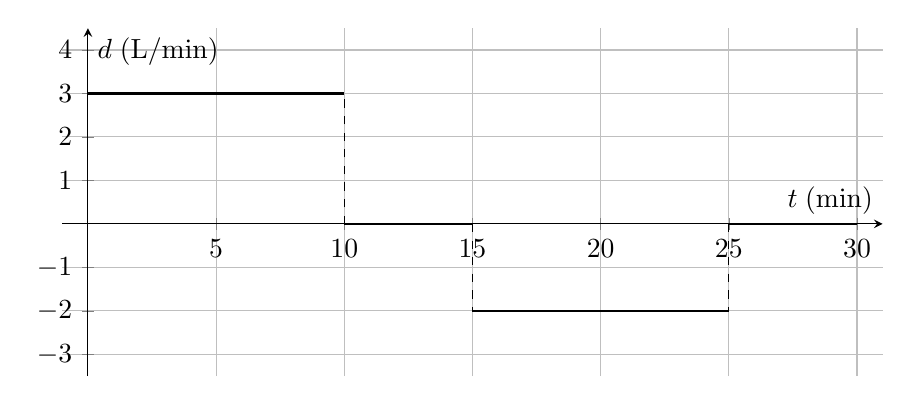
\begin{tikzpicture}
\begin{axis}[
    axis lines=middle,
    xmin=-1, xmax=31,
    ymin=-3.5, ymax=4.5,
    xlabel={$t\;(\mathrm{min})$},
    ylabel={$d\;(\mathrm{L/min})$},
    xtick={0,5,10,15,20,25,30},
    ytick={-3,-2,-1,0,1,2,3,4},
    grid=both,
    width=12cm,
    height=6cm
]
    \addplot[black,thick] coordinates {(0,3) (10,3)};
    \addplot[black,thick] coordinates {(10,0) (15,0)};
    \addplot[black,thick] coordinates {(15,-2) (25,-2)};
    \addplot[black,thick] coordinates {(25,0) (30,0)};

    \draw[dashed] (axis cs:10,0)--(axis cs:10,3);
    \draw[dashed] (axis cs:15,0)--(axis cs:15,-2);
    \draw[dashed] (axis cs:25,0)--(axis cs:25,-2);
\end{axis}
\end{tikzpicture}
\end{center}

\begin{question}
Hoeveel vloeistof zit er na \(10\) minuten in de tank?

\begin{oplossing}

Van \(t=0\) tot \(t=10\) is het debiet constant en gelijk aan

\[
3\ \mathrm{L/min}.
\]

De toegevoegde hoeveelheid is dus

\[
3\cdot10=30\ \mathrm L.
\]

De tank bevatte aanvankelijk \(15\) liter, zodat

\[
V(10)=15+30=\boxed{45\ \mathrm L}.
\]

\end{oplossing}
\end{question}

\begin{question}
Hoeveel vloeistof zit er na \(20\) minuten in de tank?

\begin{oplossing}

Na \(10\) minuten bevat de tank \(45\) liter. Tussen \(10\) en \(15\)
minuten is het debiet nul, dus het volume verandert daar niet.

Van \(15\) tot \(20\) minuten is het debiet \(-2\ \mathrm{L/min}\).
In \(5\) minuten is de verandering

\[
(-2)\cdot5=-10\ \mathrm L.
\]

Daarom

\[
V(20)=45-10=\boxed{35\ \mathrm L}.
\]

\end{oplossing}
\end{question}

\begin{question}
Hoeveel vloeistof zit er na \(25\) minuten in de tank?

\begin{oplossing}

Van \(0\) tot \(10\) minuten wordt \(30\) liter toegevoegd.

Van \(15\) tot \(25\) minuten verdwijnt

\[
2\cdot10=20\ \mathrm L.
\]

De nettoverandering is dus

\[
30-20=10\ \mathrm L.
\]

Met de beginhoeveelheid van \(15\) liter:

\[
V(25)=15+10=\boxed{25\ \mathrm L}.
\]

\end{oplossing}
\end{question}

\end{oefening}


% ------------------------------------------------------------
% OEFENING 8
% ------------------------------------------------------------

\begin{oefening}[Verplaatsing en afgelegde weg]{\oefU\ESS}

Een wandelaar beweegt eerst \(20\) minuten met een constante snelheid
van \(6\,\mathrm{km/h}\) in de positieve richting. Daarna keert hij om
en wandelt hij \(10\) minuten met een snelheid van
\(-3\,\mathrm{km/h}\).

\begin{question}
Bepaal de verplaatsing.

\begin{oplossing}

We zetten de tijden eerst om naar uren:

\[
20\,\mathrm{min}=\frac13\,\mathrm h,
\qquad
10\,\mathrm{min}=\frac16\,\mathrm h.
\]

Tijdens het eerste deel is de verplaatsing

\[
6\cdot\frac13=2\ \mathrm{km}.
\]

Tijdens het tweede deel beweegt de wandelaar in de tegengestelde
richting:

\[
(-3)\cdot\frac16=-\frac12\ \mathrm{km}.
\]

De totale verplaatsing is

\[
\Delta x
=
2-\frac12
=
\boxed{1.5\ \mathrm{km}}.
\]

\end{oplossing}
\end{question}

\begin{question}
Bepaal de afgelegde weg.

\begin{oplossing}

Voor de afgelegde weg tellen we beide trajecten positief op:

\[
s
=
2+\frac12
=
\boxed{2.5\ \mathrm{km}}.
\]

Het verschil met de verplaatsing is dat de terugweg hier niet wordt
afgetrokken.

\end{oplossing}
\end{question}

\end{oefening}


% ------------------------------------------------------------
% OEFENING 9
% ------------------------------------------------------------

\begin{oefening}[Redeneer zonder exact te rekenen]{\oefU\ESS}

Voor een functie \(f\) op \([a,b]\) is het gebied boven de \(x\)-as
groter dan het gebied onder de \(x\)-as.

Wat kun je besluiten over de georiënteerde oppervlakte?

\begin{oplossing}

Het gebied boven de \(x\)-as levert een positieve bijdrage en het gebied
onder de \(x\)-as een negatieve bijdrage.

Omdat de positieve oppervlakte groter is dan de negatieve oppervlakte
in absolute waarde, blijft er een positieve netto-bijdrage over.

Dus

\[
\boxed{S_{\mathrm{geo}}>0}.
\]

De afzonderlijke oppervlakten hoeven niet exact berekend te worden om
het teken te bepalen.

\end{oplossing}

\end{oefening}


% ------------------------------------------------------------
% OEFENING 10
% ------------------------------------------------------------

\begin{oefening}[Analyseer de redenering]{\oefU\ESS}

Een leerling zegt:

``De georiënteerde oppervlakte is nul. De grafiek moet dus overal op de
\(x\)-as liggen.''

Analyseer deze uitspraak.

\begin{oplossing}

De uitspraak is fout.

Een georiënteerde oppervlakte van nul betekent alleen dat de totale
positieve en negatieve bijdragen elkaar precies opheffen.

Als bijvoorbeeld

\[
S_+=S_-,
\]

dan geldt

\[
S_{\mathrm{geo}}
=
S_+-S_-
=
0,
\]

ook al liggen er wel degelijk gebieden boven en onder de \(x\)-as.

De grafiek hoeft dus niet overal samen te vallen met de \(x\)-as.

\end{oplossing}

\end{oefening}


% ============================================================
% GEVORDERD
% ============================================================




% ------------------------------------------------------------
% OEFENING 11
% ------------------------------------------------------------

\begin{oefening}[Ontwerp zelf een grafiek]{\oefG}

Teken een stukgewijs lineaire grafiek op het interval \([0,8]\) waarvoor:

\begin{itemize}
    \item de gewone totale oppervlakte gelijk is aan \(20\);
    \item de georiënteerde oppervlakte gelijk is aan \(4\);
    \item de grafiek zowel boven als onder de \(x\)-as ligt.
\end{itemize}

Motiveer met berekeningen dat jouw grafiek aan alle voorwaarden voldoet.

\begin{oplossing}

Noem de totale gewone oppervlakte boven de \(x\)-as \(S_+\) en de totale
gewone oppervlakte onder de \(x\)-as \(S_-\).

Uit de gewone totale oppervlakte volgt

\[
S_+ + S_-=20.
\]

Uit de georiënteerde oppervlakte volgt

\[
S_+-S_-=4.
\]

We lossen het stelsel op. Optellen geeft

\[
2S_+=24,
\]

dus

\[
S_+=12.
\]

Daaruit volgt

\[
S_-=20-12=8.
\]

Een mogelijke grafiek bestaat uit een rechthoek boven de \(x\)-as op
\([0,4]\) met hoogte \(3\), en een rechthoek onder de \(x\)-as op
\([4,8]\) met hoogte \(-2\).

Dan

\[
S_+=4\cdot3=12
\]

en

\[
S_-=4\cdot2=8.
\]

Dus

\[
S_{\mathrm{opp}}=12+8=20
\]

en

\[
S_{\mathrm{geo}}=12-8=4.
\]

Een mogelijke grafiek is:

\begin{center}
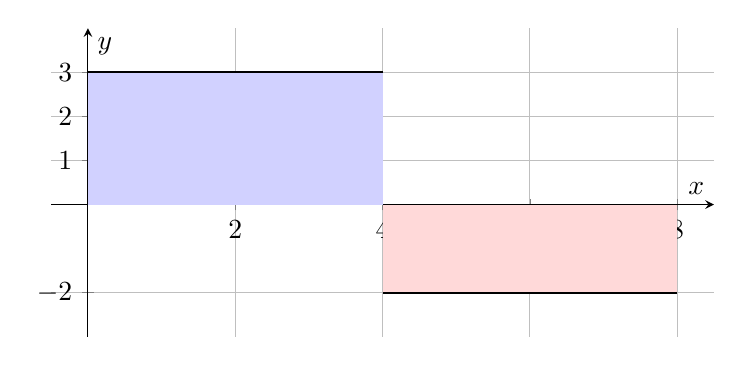
\begin{tikzpicture}
\begin{axis}[
    axis lines=middle,
    xmin=-0.5, xmax=8.5,
    ymin=-3, ymax=4,
    xlabel={$x$},
    ylabel={$y$},
    xtick={0,2,4,6,8},
    ytick={-2,0,1,2,3},
    grid=both,
    width=10cm,
    height=5.5cm
]
    \draw[fill=blue!18,draw=none]
        (axis cs:0,0) rectangle (axis cs:4,3);
    \draw[fill=red!15,draw=none]
        (axis cs:4,0) rectangle (axis cs:8,-2);

    \addplot[black,thick] coordinates {(0,3) (4,3)};
    \addplot[black,thick] coordinates {(4,-2) (8,-2)};
\end{axis}
\end{tikzpicture}
\end{center}

Er bestaan uiteraard nog veel andere correcte antwoorden.

\end{oplossing}

\end{oefening}


% ------------------------------------------------------------
% OEFENING 12
% ------------------------------------------------------------

\begin{oefening}[Van kromme grafiek naar een nieuwe methode]{\oefG}

Beschouw

\[
f(x)=x^2+1
\]

op \([0,3]\).

\begin{question}
Leg uit waarom je de oppervlakte onder de grafiek niet rechtstreeks als
één rechthoek, driehoek of trapezium kunt berekenen.

\begin{oplossing}

De bovengrens van het gebied is de grafiek van

\[
f(x)=x^2+1,
\]

en die grafiek is een kromme.

Een rechthoek, driehoek of trapezium heeft rechte zijden. Het gebied
onder de parabool is dus geen van deze gekende vlakke figuren.

Daarom kunnen we de oppervlakte niet rechtstreeks met één gewone
oppervlakteformule bepalen.

\end{oplossing}
\end{question}

\begin{question}
Verdeel \([0,3]\) in drie intervallen met gelijke breedte en gebruik
rechthoeken waarvan de hoogte telkens de functiewaarde aan het linker
uiteinde is. Bereken de som van hun oppervlakten.

\begin{oplossing}

De lengte van het interval is

\[
3-0=3.
\]

We verdelen dit in drie gelijke delen:

\[
\Delta x=\frac{3}{3}=1.
\]

De deelintervallen zijn

\[
[0,1],\qquad [1,2],\qquad [2,3].
\]

We gebruiken telkens het linker eindpunt. De hoogtes zijn dus

\[
f(0)=0^2+1=1,
\]

\[
f(1)=1^2+1=2,
\]

en

\[
f(2)=2^2+1=5.
\]

De rechthoeksoppervlakten zijn

\[
1\cdot1=1,\qquad
2\cdot1=2,\qquad
5\cdot1=5.
\]

De som is

\[
1+2+5=\boxed{8}.
\]

Omdat \(f\) stijgt op \([0,3]\), liggen deze linkerrechthoeken onder de
grafiek. De waarde \(8\) is hier dus een onderschatting van de werkelijke
oppervlakte.

\end{oplossing}
\end{question}

\begin{question}
Wat verwacht je dat er met de benadering gebeurt als je meer en smallere
rechthoeken gebruikt?

\begin{oplossing}

Als we het interval in meer deelintervallen verdelen, wordt elke
rechthoek smaller.

Daardoor volgt de bovenkant van de rechthoeken de kromme steeds beter en
wordt de afwijking tussen de rechthoeken en de werkelijke grafiek kleiner.

We verwachten dus dat de benadering steeds nauwkeuriger wordt.

Dit idee wordt in het volgende hoofdstuk verder ontwikkeld en leidt naar
Riemannsommen, limieten en uiteindelijk de bepaalde integraal.

\end{oplossing}
\end{question}

\end{oefening}





\end{document}

